\chapter{Cluster Cosmology}
\label{ch:clusters}
\section{Overview}
%As described in the last chapter, on average the universe is homogenous - the expansion history, mean energy densities are reasonably well understood, at least empirically. However, the inhomogenities in the universe in the form of large scale structures such as galaxies, cluster of galaxies etc., carry a wealth of cosmological information. Given that ~85\% of matter in the universe is made up of cold dark matter, the growth of cosmic structure can be attributed to two main factors mainly: gravitational growth of initial density perturbations controlled by expansion of space and baryonic physics. According to inflationary paradigm and also observationally corroborated by CMB data, the initial density perturbations are scale independent. The matter distribution at late times can be probed by number of different observations: galaxy redshift surveys, weak gravitational lensing, galaxy cluster abundance; latter being the focus of this chapter.  %The chapter is organised as follows: in ~\ref{growth} I discuss the growth density perturbations during various regimes, followed by density power spectrum in ~\ref{density_ps}. In ~\ref{stats}, I explain the statistics of collapsed objects
In the last chapter, I introduced the CMB anisotropies which are sourced by small pertrubations of density in the early Universe.
With time and gravity, these initially tiny perturbations grow to become galaxies, galaxy clusters etc.,
This process of structure growth yields a plethora of tests of the cosmological model.
\section{Linear theory of structure formation}
\label{growth}
In this section, I will describe the evolution of matter density perturbations in the linear regime. This section closely follows Ryden 2003.
Assuming that universe is filled with pressure less matter with mean mass density $\rho_{m}(t)$. 
%As we saw in the last chapter, mass density is related to scale parameter as $\rho_{m}(t) \propto a^{-3}(t)$. 
By inducing a small density fluctuation ($\delta \ll 1$) within a region of spherical radius `R'
\begin{equation}
\rho(t) = \rho_{m}(t)(1+\delta).
\end{equation}
 The gravitational pull on the outer shell of the sphere is given by%at the tip of the spherical region is given by 
\begin{equation}
\ddot{R} = -\frac{GM}{R^{2}}
\label{clus_accel}
\end{equation} 
where $M = 4 \pi /3 \: \rho R^{3}$ is the total mass within the sphere, we can rewrite Eqn. ~\ref{clus_accel}
\begin{equation}
\frac{\ddot{R}}{R}= -\frac{4\pi}{3} G\rho_{m} - \frac{4\pi}{3} G \rho_{m} \delta. 
\end{equation}
As the sphere expands the mass within the sphere is conserved
\begin{equation}
M = \frac{4\pi}{3} \rho_{m}(t)[1+\delta(t)]R(t)^{3}.
\end{equation}
From which we get 
\begin{equation}
R(t) \propto \rho_{m}(t)^{-1/3}[1+\delta(t)]^{-1/3}.
\end{equation}
Since $\rho_{m} \propto a^{-1/3}$ in an expanding universe,
\begin{equation}
R(t) \propto a(t)[1+\delta(t)]^{-1/3}.
\end{equation}
Taking two time derivatives of the above equation we get
\begin{equation}
\frac{\ddot{R}}{R}  = \frac{\ddot{a}}{a} - \frac{1}{3}\ddot{\delta} - \frac{2\dot{a}}{3a} \dot{\delta} .
\end{equation}
Rearranging the above equations we get 
\begin{equation}
\frac{\ddot{a}}{a} - \frac{1}{3}\ddot{\delta} - \frac{2\dot{a}}{3a} \dot{\delta} = -\frac{4 \pi}{3} G\rho_{m} (1-\delta).
\label{eq1}
\end{equation}
%$\frac{\ddot{a}}{a}$ is the expansion of the background universe, substituting $\delta = 0$ in the above equation we get
We now want to split this up between the dynamics of the unperturbed universe ($\delta =0 $) and perturbation
\begin{equation}
\frac{\ddot{a}}{a}  = -\frac{4 \pi}{3} G\rho_{m}.
\end{equation}
Substituting the above relation in Eqn. ~\ref{eq1} yields 
\begin{equation}
- \frac{1}{3}\ddot{\delta} - \frac{2\dot{a}}{3a} \dot{\delta}  = -\frac{4 \pi}{3} G\rho_{m}\delta,
\end{equation}
or
\begin{equation}
\ddot{\delta} + 2 H\dot{\delta} = 4\pi G \rho_{m} \delta.
\end{equation}
Considering the relativistic corrections the above equation changes to 
\begin{equation}
\ddot{\delta} + 2 H \dot{\delta} = \frac{4\pi G}{c^{2}} \rho_{m} \delta.
\label{eq2}
\end{equation}
In the early radiation dominated phase of the universe $\Omega_{m} \ll 1$ and $H = 1/(2t)$ which results in 
\begin{equation}
\ddot{\delta} + \frac{1}{t} \dot{\delta} \approx 0,
\end{equation}
solving which we get,
\begin{equation}
\delta(t) \approx C_{1} + C_{2} lnt
\end{equation}
During the radiation dominated epoch, baryon density oscillated as baryons and photons were tightly coupled. 
Whereas the dark matter density grew at a logarithmic rate as predicted by the above equation.  
Similarly, during the dark energy dominated epoch Eqn. ~\ref{eq2} takes the form
\begin{equation}
\ddot{\delta} + 2 H_{\Lambda} \dot{\delta} \approx 0
\end{equation}
which results in
\begin{equation}
\delta(t) \approx D_{1} + D_{2}e^{-2H_{\Lambda} t}.
\end{equation}
Dark matter density perturbation exponentially decays off in dark energy dominated epoch. 


During the matter dominated epoch, density perturbations follow
\begin{equation}
\ddot{\delta} + \frac{4}{3t} \dot{\delta} -\frac{2}{3t^{2}} \delta = 0.
\end{equation}  
Assuming a power law solution of the form $Dt^{n}$  and plugging it in above equation we get
\begin{equation}
\delta(t) \approx D_{1} t^{2/3} + D_{2} t^{-1}.
\end{equation}
Thus during matter domination matter perturbation grow as $t^{2/3}$. Given these different dynamics, studying how density perturbations grow can yield strong tests of cosmology and the constituents of the Universe. 
\section{Power spectrum}
\label{density_ps}
In Fourier space the perturbations can be written as 
\begin{equation}
\delta_{k} = \frac{1}{V} \int^{\infty}_{0} \delta(x) e^{ik.x} d^{3}x .
\end{equation}
The matter power spectrum and auto correlation are related as follows:
\begin{equation}
\langle \delta(x) \delta^{*}(x) \rangle = \int^{\infty}_{0} \frac{dk}{k} \frac{k^{3} |\delta^{2}(k)|}{2\pi^{2}} = \int^{\infty}_{0} \frac{dk}{k}\frac{k^{3} P(k)}{2\pi^{2}}
\end{equation}
where by definition $P(k) = |\delta^{2}(k)|$.
In the inflationary paradigm, the primordial fluctuations are quantum fluctuations that have been blown up to macroscopic scale by inflation. 
%As proposed by Harrison and Zel'dovich, these primordial fluctuations are scale-invariant \footnote{ otherwise it would imply a preferred mass scale for fluctuations entering the horizon}
In inflationary models, this primordial fluctuations are nearly scale invariant, since inflation has no preferred scale,
\begin{equation}
P_{primordial}(k) \propto k
\end{equation}

\begin{figure}[H]
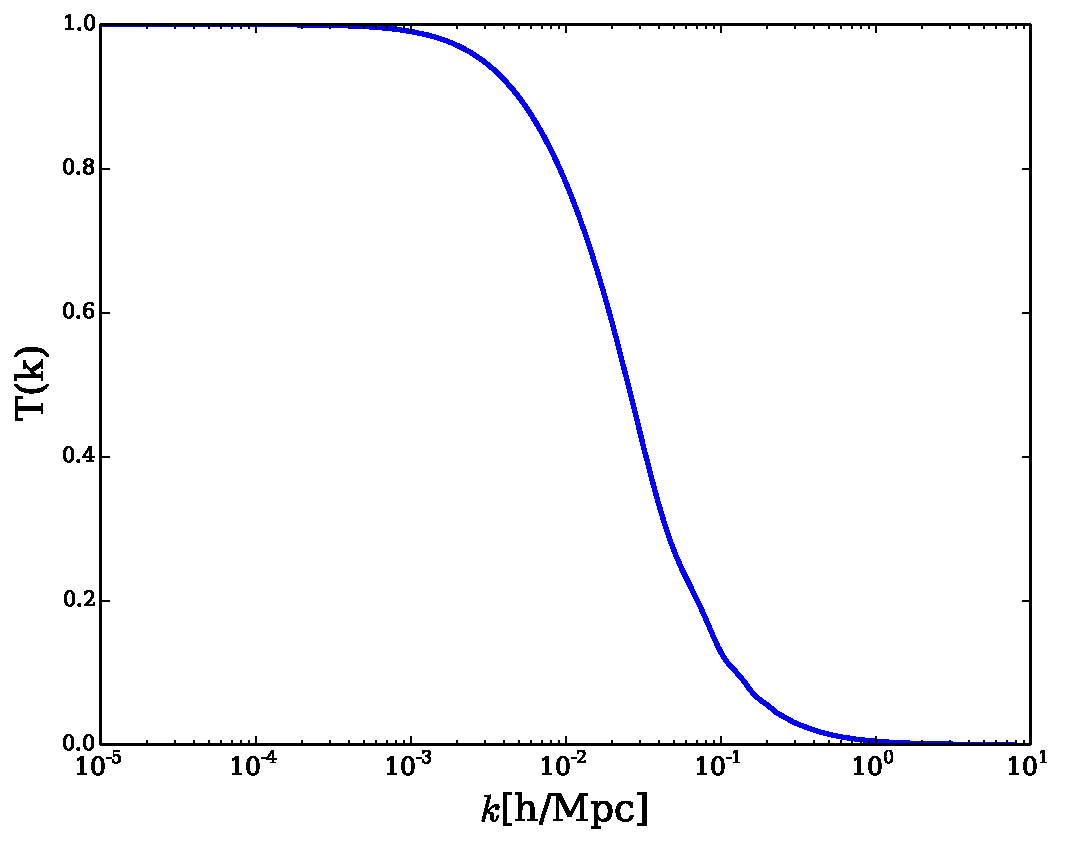
\includegraphics[width = \columnwidth]{figs/tf.pdf}
\caption{Total transfer function (CDM+baryon+neutrinos) as calculated by $CAMB$.}
\label{tf}
\end{figure}

The primordial densities grow in a complicated way as explained in the previous section; the evolved matter power spectrum can be written as fucntion redshift and wave number as
\begin{equation}
P(k,z) = P_{primordial} (k) D(z)^{2} T(k,z)^{2}
\end{equation}
where D(z) is the growth factor and T(k,z) is the transfer function. 
Growth factor for cold dark matter is given by
\begin{equation}
D(z) = H(z) \int^{\infty}_{z} \frac{dz'(1+z')}{H^{3}(z')}.
\end{equation}
The transfer function depends on the complex interactions between various components in the universe. 
While there are approximated expression for transfer function, however, the exact solution of the transfer function can only be obtained numerically. 
Numerical codes such as CAMB, CLASS etc., solve the multi -component Boltzmann equations to provide T(k,z) for a given set of parameters. 

The shape of transfer function gives insight into the growth of perturbations. At early phase of the universe during radiation dominated epoch, super horizon scales grew according to the growth factor D(z) as the transfer function is unity. However, sub horizon perturbations grow only logarithmically; smaller modes entered horizon earlier than longer modes, hence had more logarithmic growth. After matter-radiation equality, perturbations grew equally on all scales. The wiggles in the transfer function at intermediate scales is due to Baryon Acoustic Oscillations (BAO). Before recombination, photons and baryons were tightly coupled, baryons experienced two opposing forces: gravitational pull due to dark matter potential well and pressure due to the radiation component resulting in oscillations of photon-baryon plasma. However, at recombination photons-baryons decouple and the baryon perturbations evolve according to the background universe. This length scale can be used as a standard ruler to measure the geometry of the universe \cite{chang07}.

Fig. ~\ref{fig_ps} shows the matter power spectrum at two different redshifts for $Planck$ 2018 cosmological parameters.The power at large scales i.e., $k<k_{eq}$ obtained by multiplying the primordial power spectrum with growth factor (as transfer function is unity at those scales). As one expects, the maximum of the power spectrum is directly linked to the horizon at matter-radiation equality, $k_{eq} = 0.01$.  

\begin{figure}[H]
\includegraphics[width = \columnwidth]{figs/ps.pdf}
\caption{Total matter power spectrum generated by $CAMB$ for two different redshifts.}
\label{fig_ps}
\end{figure}

\section{Statistics of spherically collapsed objects}
\label{stats}
In the previous sections we introduced equations for density perturbations in both real and Fourier space. However, in practice, we observe the density perturbation averaged over a given volume which we define as 'density contrast'. Mathematically, density contrast within a radius `R' is given by
\begin{eqnarray}
\Delta(x, R) = \int d^{3}x' W(|x' - x|) \delta(x') \\
\Delta(k, R) = W(k,R) \delta(k)
\end{eqnarray}
The variation in the observed density contrast in a sphere of radius R is given by
\begin{equation}
\sigma^{2}(R) = \langle \Delta^{2}(x,R) \rangle = \int d lnk \nabla^{2}(k) |W(k,R)|^{2}
\end{equation}
where $\nabla(k) = \sqrt{k^{3}P(k)/2\pi^{2}}$ is the dimensionless power spectrum.
%\begin{equation}
%\nabla^{2}(k) = \frac{k^{3}P(k)}{2\pi^{2}}
%\end{equation}
Assuming that the density field follows Gaussian random distribution, which is well supported by observation. The probability that the sphere of radius, R, has density contrast $\delta$ is given by
\begin{equation}
P(\Delta, R) = \frac{1}{\sqrt(2 \pi \sigma^{2}(R))} exp(-\frac{\delta^{2}}{2\sigma^{2}(R)}) d\delta.
\end{equation}
It is important to note here that we can also express $P(\Delta, R) = P(\Delta, M)$, where R is related to M as $M = \frac{4\pi}{3} R^{3}$
\subsection{The Press-Schechter Theory}
\label{halo-theory}
In 1974 Press-Schechter came up with a simple model to predict the number of dark matter halos \citep{press74}. The basic idea is that a sphere of radius `R' with density contrast $\Delta$ will form a dark matter if $\Delta$ greater than a critical value $\Delta_{c}$. The probability of finding dark matter halos with mass greater than M is given by
\begin{equation}
F(M) = \int^{\infty}_{\Delta_{c}} P(\Delta, M) d\Delta = \frac{1}{2} erfc(\frac{\nu}{\sqrt(2)})
\end{equation}
where $\nu = \Delta_{c}/ \sigma(M)$. The halo mass function, i.e, the number density of halos between mass M and M+dM is given by 
\begin{equation}
\frac{dn(M,z)}{dM} = -\sqrt{\frac{2}{\pi}} \frac{\rho_{m}}{M} \frac{\Delta_{c}}{\sigma^{2}(M,z)} \frac{d\sigma(M,z)}{dM}  exp(-\frac{\Delta^{2}_{c}}{2 \sigma^{2}(M,z)}).
\label{eq_press-shcech}
\end{equation}
The above equation predicts too many low-mass halos and too few high-mass halos compared to the N-body simulations. 
For precise cosmological applications, current estimates of the halo mass function rely on some form of Eqn. ~\ref{eq_press-shcech} with some additional fitting parameters to achieve a better fit, for example \cite{tinker08, jenkins01}.

\section{Galaxy Clusters \& Cosmology}
\subsection{Galaxy Clusters}
According to the standard model of cosmology, galaxy clusters are the largest and most recent gravitationally collapsed objects to form because structure grows hierarchically. 
A galaxy cluster contains hundreds to thousands of galaxies that are bound together by gravity.
These are very massive objects with typical masses ranging from $10^{14} - 10^{15} $ times the mass of Sun ($M_{\odot}$). %\footnote{Virial radius corresponds to the radius of a spherical region which is sufficiently over dense with respect to the background density that it will detach from the Hubble expansion and start collapsing to form a structure}.
The majority the mass is in the form of invisible dark matter (80-87\%), which generally follows a spherically symmetric Navarro-Frenk-White (NFW) model  \citep{navarro97}. 
Around 12\% of the cluster mass is in the form of hot intracluster medium (ICM)- a sparse hot plasma that fills the cluster. 
The temperature of the ICM is of order ten million Kelvin and thus the ICM predominantly emits X-rays. 
The remaining 2\% of the cluster mass is in the form of stars, cold gas, and dust in galaxies.
\begin{figure}[H]
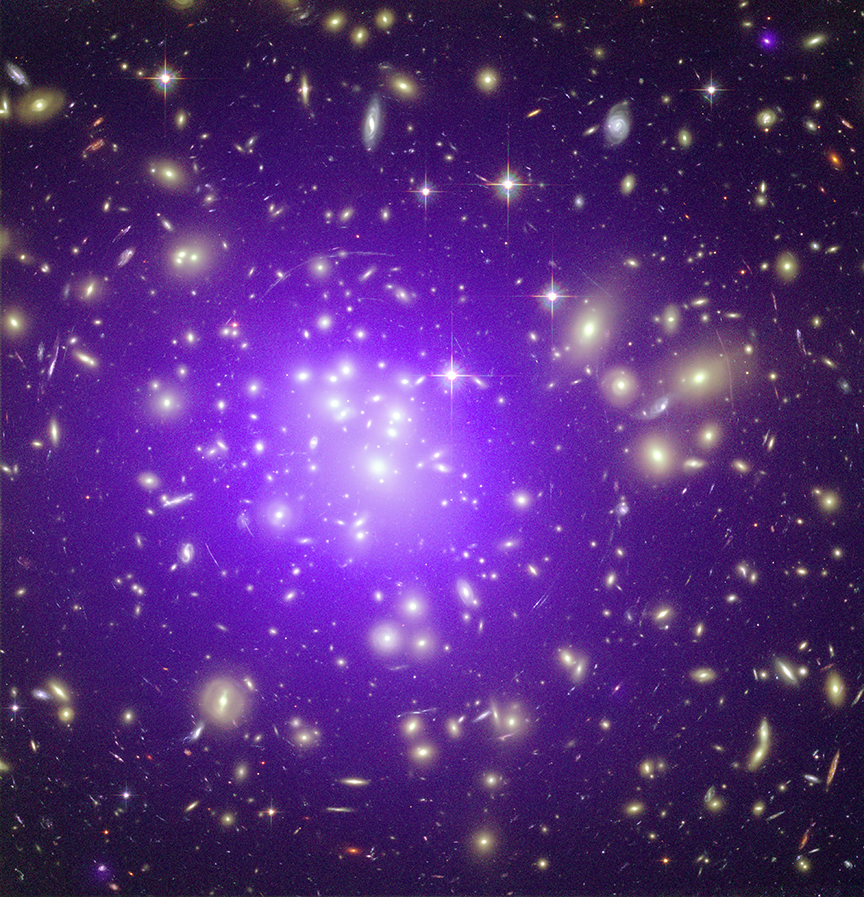
\includegraphics[width = \columnwidth]{figs/Abell_1689.jpg}
\caption{Galaxy cluster Abell 1689. Galaxy cluster are multi wavelength objects- optical galaxies are in yellow colour and X-ray emission from the hot intra cluster medium appears in purple.  Credits: HST/Chandra X-ray observatory. }
\label{cluster}
\end{figure}

Fig. ~\ref{cluster} shows the image of a galaxy cluster Abell 1689 which is in constellation Virgo. The X-ray emission due to hot ICM is shown as purple in the image; galaxies from the optical data are coloured yellow. The long arcs in the optical image is caused by distortion due to strong gravitational lensing. \\

\subsection{Cluster cosmology}
Clusters have long provided crucial information about the cosmological model. Dark matter was discovered in Coma cluster in 1930s, when Fritz Zwicky observed that galaxies in cluster were moving too fast to be held by the gravitational pull of the visible galaxies \citep{zwicky33}. In the 1990s clusters provided evidence for low matter density universe \citep{white93a}. Clusters are so large that the ratio of baryon to dark matter content in the cluster should be equal to that of universe as a whole. So, the gas mass fraction $f_{gas}$ should be equal to  $\Omega_{b} /\Omega_{m}$.
 With the values of $\Omega_{b}$ and $f_{gas}$ from baryon acoustic oscillations and X-ray observations, we can calculate $\Omega_{m}$. 
% The total baryonic mass can be calculated in rudimentary way by calculating mass of stars and hot gas in the cluster, $\Omega_{b}$ is obtained from big bang nucleosynthesis, one can constrain $\Omega_{m}$ \pending{white}.
More recently, the community has been interested in using galaxy clusters to probe dark energy, neutrinos and cosmic growth of structure \citep{allen11,mantz08,mantz10a,mantz15,dehaan16,bocquet18,rozo10,vikhlinin09,salvati17,zubeldia19}.


Galaxy clusters are powerful probes of dark energy. The dark energy effects the evolution of universe in two different ways. 
First, it accelerates the expansion of the universe and thus slowing down the structure formation. Second, it affects the volume of the survey. Cluster number counts is sensitive to both of these effects: the abundance and the correlation function of galaxy clusters depend on the volume surveyed and rate of structure growth. Fig. \ref{de_plot} shows the cluster number count as a function of redshift for various dark energy equation of state parameters, $w$, and for fixed dark energy density parameter, $\Omega_{E}$. For fixed dark energy density, $\Omega_{E}$, and less negative $w$ implies less acceleration and thus higher velocity in the past. 
This results in few clusters at low redshift due to decreased volume surveyed and more clusters at high redshift due to decreased structure growth \citep{mohr03}.
\begin{figure}[H]
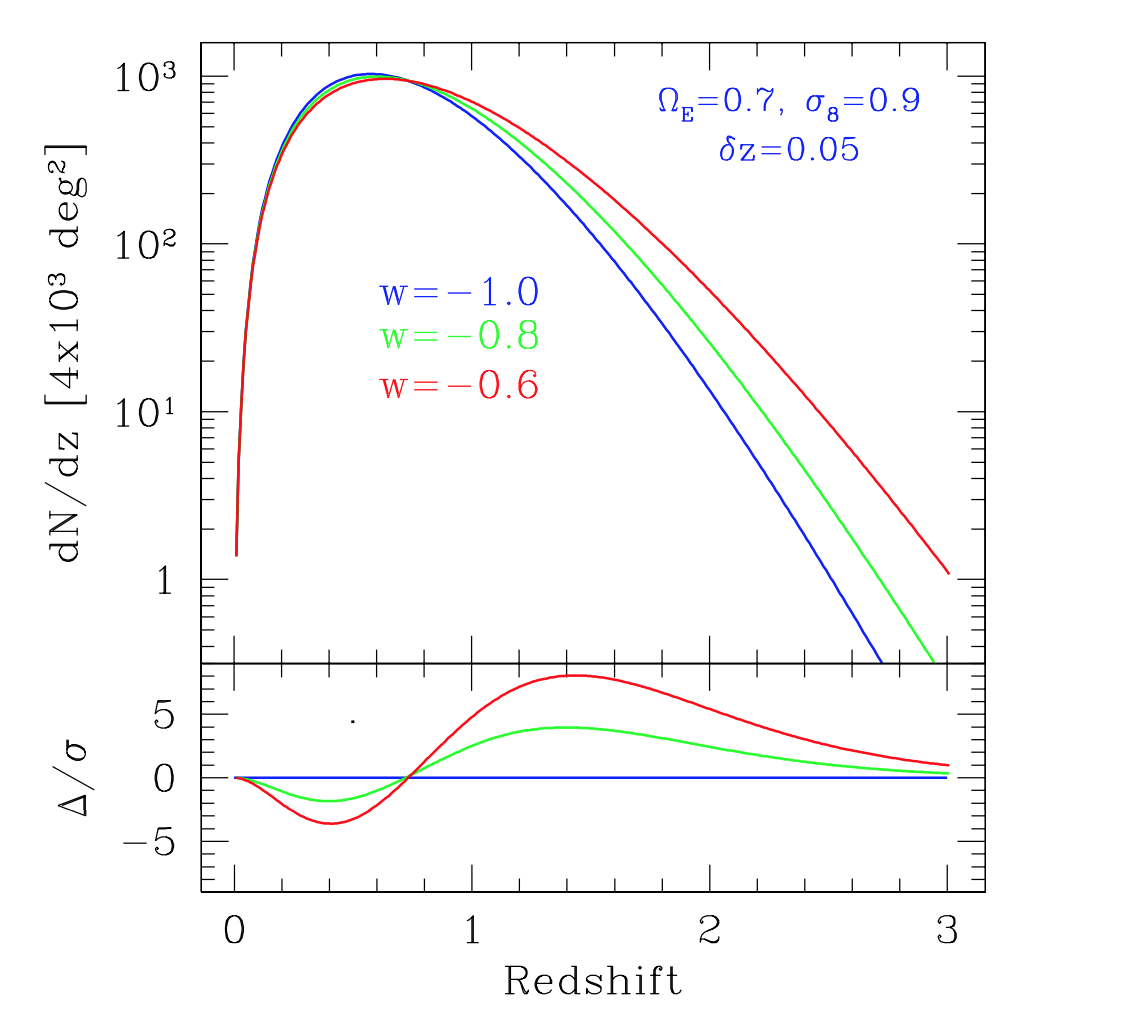
\includegraphics[width = \columnwidth]{figs/cluster_de_plot.png}
\caption{The cluster count redshift distribution for a simulated 4000 deg$^{2}$ survey. On the top panel three models with different dark energy equation of state parameters are shown and statistical differences are quantified in the bottom panel \citep{mohr03}. }
\label{de_plot}
\end{figure}


As seen in ~\S\ref{halo-theory}, halo/cluster abundance as a function of mass is sensitive to cosmological parameter such as $\Omega_{m}$ and $\sigma_{8}$. 
Constraints obtained on $\Omega_{m}$, $\sigma_{8}$, and dark energy equation of state parameter, $w$, is shown in Fig ~\ref{clustercosmology}.
As can be inferred from the plot, cluster constraints are complementary to that of CMB anisotropies. For the above constraints, only 241 clusters from ROSAT all sky survey were used \citep{mantz15}. Given that ongoing and future surveys will detect tens to hundreds of thousands of galaxy clusters, clusters will become indispensable probes of cosmology \citep{so18, bender18, lsst09,erosita12,cmbs4-sb1}. %While the clusters are powerful probes of cosmology, the key issued the fidelity of the mass tracer. 

\begin{figure}[H]
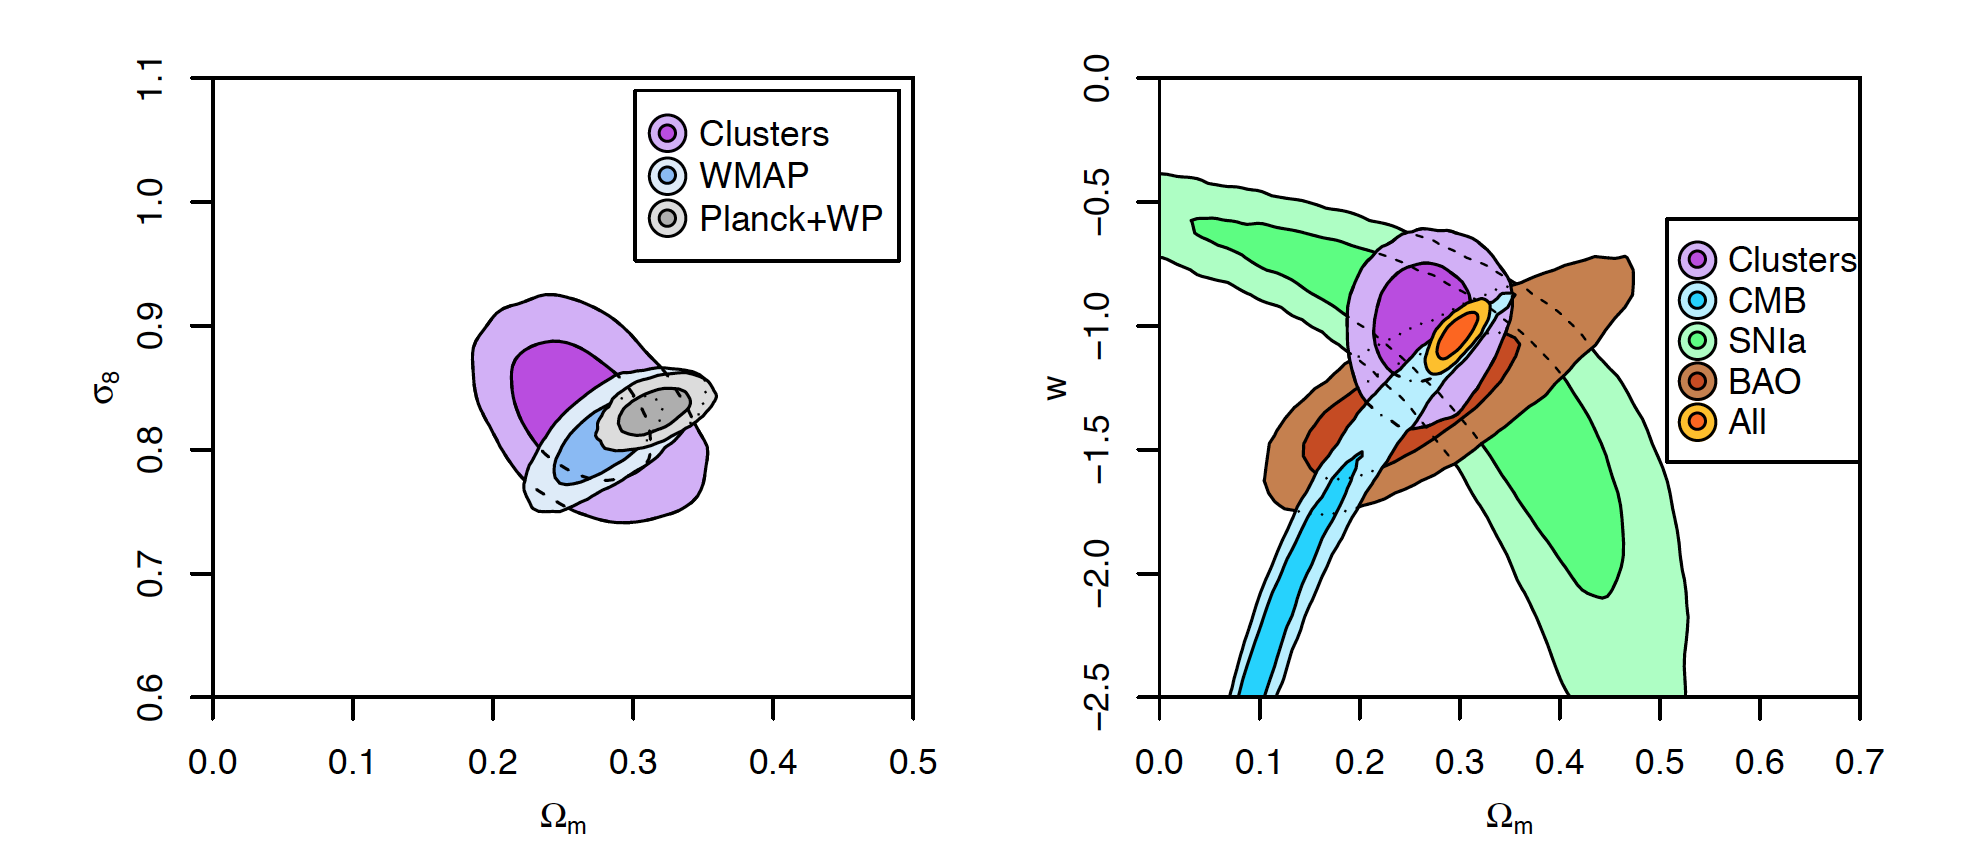
\includegraphics[width = \columnwidth]{figs/cosmology.png}
\caption{On the left is flat $\Lambda$CDM model: constraints on $\Omega_{m}$ and $\sigma_{8}$ from clusters in purple, from CMB observations in blue ($Planck$) and grey ($Planck$ and WMAP). On the right we have flat $w$CDM: constraints on $w$ and $\Omega_{m}$ for various cosmological probes. Cluster (purple) provide the tightest single-probe constraints \citep{mantz15}.  }
\label{clustercosmology}
\end{figure}
\subsection{Cluster cosmology is limited by mass estimation}

While clusters are powerful probes of cosmology, the use of clusters for cosmology is currently limited by the fidelity of the mass estimation. Many ways to measure the cluster mass relate a cluster observable $'O'$ to the cluster mass through a parametric relation 
\begin{equation}
O = A M^{B} f(z)^{C} +D
\label{obs-mass}
\end{equation} 
where A is the normalisation parameter, D is the intrinsic scatter, B and C are the mass and redshift evolution parameters respectively. The trouble is that these depend on complicated baryonic physics which is not well understood and any error in the estimated mass will affect the inferred constraints from cluster cosmology. 
\begin{figure}[H]
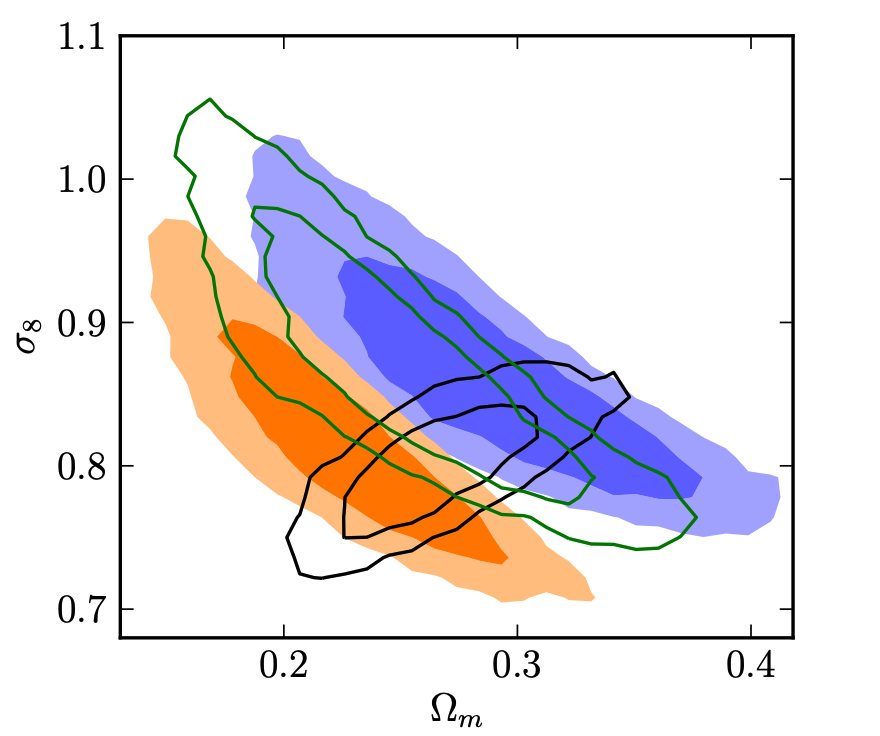
\includegraphics[width = \columnwidth]{figs/mass_cosmology.png}
\caption{Effects of systematics in mass estimation on cluster cosmology. Constraints on matter fluctuation amplitude parameter ($\sigma_{8}$) and matter density parameter ($\Omega_{m}$) from CMB data is shown in black contour. The coloured counters (orange, green, and blue) are the constraints obtained using cluster counts for three different mass observable scaling relation. }
\label{m_cosmo}
\end{figure}
Fig. ~\ref{m_cosmo} shows the systematic effects of cluster mass estimation on cosmological parameters $\Omega_{m}$ and $\sigma_{8}$. The black contour represents the cosmological constraints obtained using CMB.
The green, blue, and orange contours represent constraints due to cluster number count for three different mass-observable scaling relations.
While cluster number counts provide complementary constraints to that of CMB, however, any systematic in mass estimation will eventually lead to uncertainties in cosmological parameters \citep{hasselfield13}. 


Accurate cluster mass estimates are essential to fully realise the potential of cluster cosmology.
One of the ways to obtain robust cluster masses is through weak gravitational lensing \citep{becker10}. 
Unlike the mass observable scaling relation, cluster mass estimation through lensing of a background source is independent of baryonic physics and directly probes the total mass distribution in the galaxy cluster. 
While lensing is nearly unbiased, it is weak to provide mass of single galaxy cluster. Thus we use lensing to reduce the scatter in the parameters of Eq. \ref{obs-mass}.

The background source can either optical or CMB, with CMB having the following advantages over optical:
\begin{itemize}
\item CMB is at precise redshift of $z \approx 1100$, on the other hand, the probability of finding an optical source behind a high redshift ($z$ >1) galaxy cluster decreases exponentially.
\item CMB has relatively less systematics
\item the statistical properties of CMB are very studied and hence easy to model
\end{itemize}
The rest of the chapters focus on various methods we have developed to extract lensing signal from CMB data, the data used, and the results we have obtained. 
%While the background source can be any source of radiation, the focus of this thesis is on Cosmic Microwave Background.



  

 

 
 

   